% fig5b-equivalence-sheaf.tex
\documentclass[tikz,border=10pt]{standalone}
% common-styles.tex
% Shared TikZ styles for wonton-proof paper figures

\usepackage{silence}
\WarningFilter{latex}{Missing character} 
\tracinglostchars=0 % Suppress engine-level "Missing character" warnings

\usepackage{fontspec}
\usepackage{unicode-math}

% Use filenames for reliability with Tectonic
\setmainfont{LibertinusSerif-Regular.otf}[
    BoldFont=LibertinusSerif-Bold.otf,
    ItalicFont=LibertinusSerif-Italic.otf,
    BoldItalicFont=LibertinusSerif-BoldItalic.otf
]
\setsansfont{LibertinusSans-Regular.otf}[
    BoldFont=LibertinusSans-Bold.otf,
    ItalicFont=LibertinusSans-Italic.otf
]
\setmonofont{LibertinusMono-Regular.otf}

% Try a more standard math font if LibertinusMath is causing nullfont issues
\setmathfont{LibertinusMath-Regular.otf}
% \setmathfont{latinmodern-math.otf}[range=digits] 

\usepackage{amsmath}
\usepackage{tikz}
\usepackage{forest}

\usetikzlibrary{
    arrows.meta,
    calc,
    decorations.pathreplacing,
    fit,
    positioning,
    shapes.geometric,
    shapes.misc,
    backgrounds,
    shadows.blur,
    fadings
}

% Color palette (muted, print-friendly)
\definecolor{ink}{RGB}{45,45,52}
\definecolor{muted}{RGB}{115,115,125}
\definecolor{highlight}{RGB}{198,120,44}
\definecolor{accentblue}{RGB}{86,130,178}
\definecolor{accentgreen}{RGB}{84,156,132}
\definecolor{blocked}{RGB}{140,75,75}
\definecolor{goalnode}{RGB}{255,255,255}
\definecolor{terminal}{RGB}{238,239,244}
\definecolor{deadnode}{RGB}{248,245,245}
\definecolor{flowbox}{RGB}{250,250,252}
\definecolor{basin1}{RGB}{224,234,248}
\definecolor{basin2}{RGB}{246,232,221}
\definecolor{basin3}{RGB}{228,242,234}
\definecolor{heatbase}{RGB}{86,130,178}

\tikzset{
    line cap=round,
    line join=round,
    pop/.style={
        blur shadow={shadow blur steps=5, shadow blur extra rounding=1.3pt}
    },
    base node/.style={
        rounded rectangle,
        draw=ink,
        line width=0.6pt,
        fill=goalnode,
        text=ink,
        minimum width=2.2cm,
        minimum height=0.7cm,
        align=center,
        pop
    },
    goal/.style={base node, fill=goalnode},
    terminal/.style={base node, fill=terminal, line width=0.9pt},
    dead/.style={base node, fill=deadnode, dashed},
    flowbox/.style={
        rectangle,
        draw=muted,
        rounded corners=3pt,
        fill=flowbox,
        minimum width=1.8cm,
        minimum height=0.6cm,
        align=center,
        font=\normalfont\small,
        text=ink,
        pop
    },
    decision/.style={
        diamond,
        draw=muted,
        fill=flowbox,
        aspect=2.4,
        font=\normalfont\small,
        inner sep=1pt,
        text=ink
    },
    protocolbox/.style={
        rectangle,
        draw=muted,
        rounded corners=4pt,
        fill=flowbox,
        minimum width=2cm,
        minimum height=0.8cm,
        font=\normalfont\small,
        align=center,
        text=ink
    },
    tactic/.style={
        ->,
        >=Stealth,
        draw=muted,
        line width=0.75pt
    },
    tacticlight/.style={
        ->,
        >=Stealth,
        draw=muted!45,
        dashed,
        line width=0.6pt
    },
    backprop/.style={
        ->,
        >=Stealth,
        draw=muted!70,
        dashed,
        line width=0.6pt
    },
    selected/.style={
        tactic,
        draw=highlight,
        line width=1.4pt
    },
    divergetactic/.style={
        tactic,
        draw=highlight,
        line width=1.4pt
    },
    divergenode/.style={
        base node,
        draw=highlight,
        line width=1.0pt
    },
    divergeblock/.style={
        blockedtactic,
        line width=1.2pt
    },
    blockedtactic/.style={
        tactic,
        draw=blocked,
        densely dashed
    },
    flowarrow/.style={
        ->,
        >=Stealth,
        draw=muted,
        line width=0.75pt
    },
    crosslink/.style={
        -,
        draw=muted!70,
        dotted,
        line width=0.6pt
    },
    annot/.style={
        font=\normalfont\footnotesize,
        text=muted
    },
    visit/.style={
        annot,
        font=\normalfont\scriptsize
    },
    annotbg/.style={
        annot,
        fill=white,
        inner sep=1.5pt
    },
    tacticlabel/.style={
        annot,
        font=\ttfamily\footnotesize,
        text=muted
    },
    formula/.style={
        font=\normalfont\footnotesize,
        draw=muted,
        rounded corners=2pt,
        fill=white,
        inner sep=3pt
    },
    paneltitle/.style={
        font=\normalfont\bfseries,
        text=ink
    },
    trajectory/.style={
        ->,
        draw=muted!70,
        line width=0.6pt
    }
}

\begin{document}
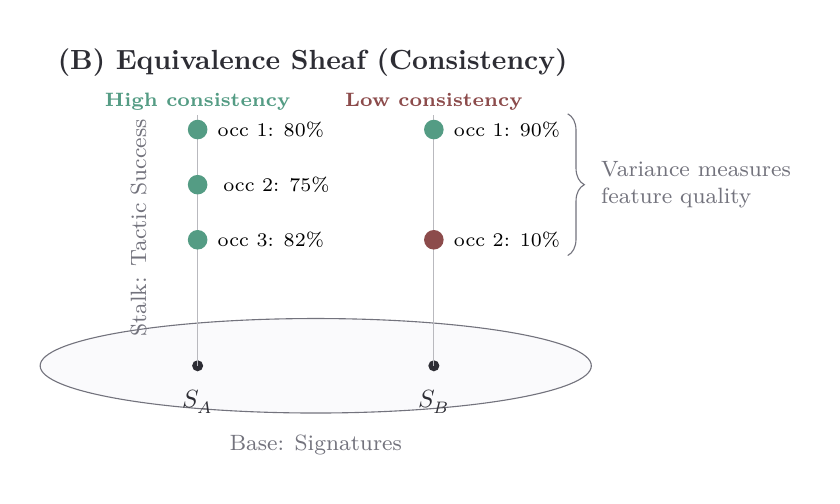
\begin{tikzpicture}[
    every node/.style={font=\small},
    show background rectangle,
    background rectangle/.style={fill=white}
]
\begin{scope}[shift={(0, 0)}]
    \node[paneltitle, anchor=south west] at (-3.4, 3.55) {(B) Equivalence Sheaf (Consistency)};
    
    % Base space (Signature)
    \draw[draw=muted, fill=flowbox] (0, 0) ellipse (3.5cm and 0.6cm);
    \node[annot, anchor=north] at (0, -0.75) {Base: Signatures};
    
    % Point S_A
    \fill[ink] (-1.5, 0) circle (2pt) node[below=0.18cm] {$S_A$};
    
    % Stalk at S_A (Fiber)
    \draw[draw=muted!50] (-1.5, 0) -- (-1.5, 3.5);
    \node[annot, rotate=90] at (-2.25, 1.75) {Stalk: Tactic Success};
    
    % Data points on stalk (Occurrences)
    % Consistent example
    \node[circle, fill=accentgreen, inner sep=2.5pt, label={right:\scriptsize occ 1: 80\%}] at (-1.5, 3.0) {};
    \node[circle, fill=accentgreen, inner sep=2.5pt, label={[xshift=2pt]right:\scriptsize occ 2: 75\%}] at (-1.5, 2.3) {};
    \node[circle, fill=accentgreen, inner sep=2.5pt, label={right:\scriptsize occ 3: 82\%}] at (-1.5, 1.6) {};
    
    \node[annotbg, text=accentgreen, font=\bfseries\scriptsize] at (-1.5, 3.35) {High consistency};

    % Point S_B (Inconsistent)
    \fill[ink] (1.5, 0) circle (2pt) node[below=0.18cm] {$S_B$};
    \draw[draw=muted!50] (1.5, 0) -- (1.5, 3.5);
    
    % Data points
    \node[circle, fill=accentgreen, inner sep=2.5pt, label={right:\scriptsize occ 1: 90\%}] at (1.5, 3.0) {};
    \node[circle, fill=blocked, inner sep=2.5pt, label={right:\scriptsize occ 2: 10\%}] at (1.5, 1.6) {};
    
    \node[annotbg, text=blocked, font=\bfseries\scriptsize] at (1.5, 3.35) {Low consistency};
    
    % Brace
    \draw[decorate, decoration={brace, amplitude=6pt}, draw=muted] (3.2, 3.2) -- (3.2, 1.4)
        node[midway, right=0.3cm, annot, align=left] {Variance measures\\feature quality};
\end{scope}\end{tikzpicture}
\end{document}
